%!TEX root = ../quantum.tex
\subsubsection{Вопрос 3}
<<<<<<< HEAD
Найдите $\Psi(p)$ по данным $\Psi(x)$. Найдите связь ширины в $x$ и $p$ представлениях. Сначала найдите нормировочный множитель $\Psi(x)=\exp{-u|x|}$
=======

 Найдите $\Psi(p)$ по данным $\Psi(x)$. Найдите связь ширины в $x$ и $p$ представлениях. Сначала найдите нормировочный множитель $\Psi(x)=\exp{-u|x|}$
>>>>>>> master

% \begin{wrapfigure}{l}{0.3\linewidth}
% 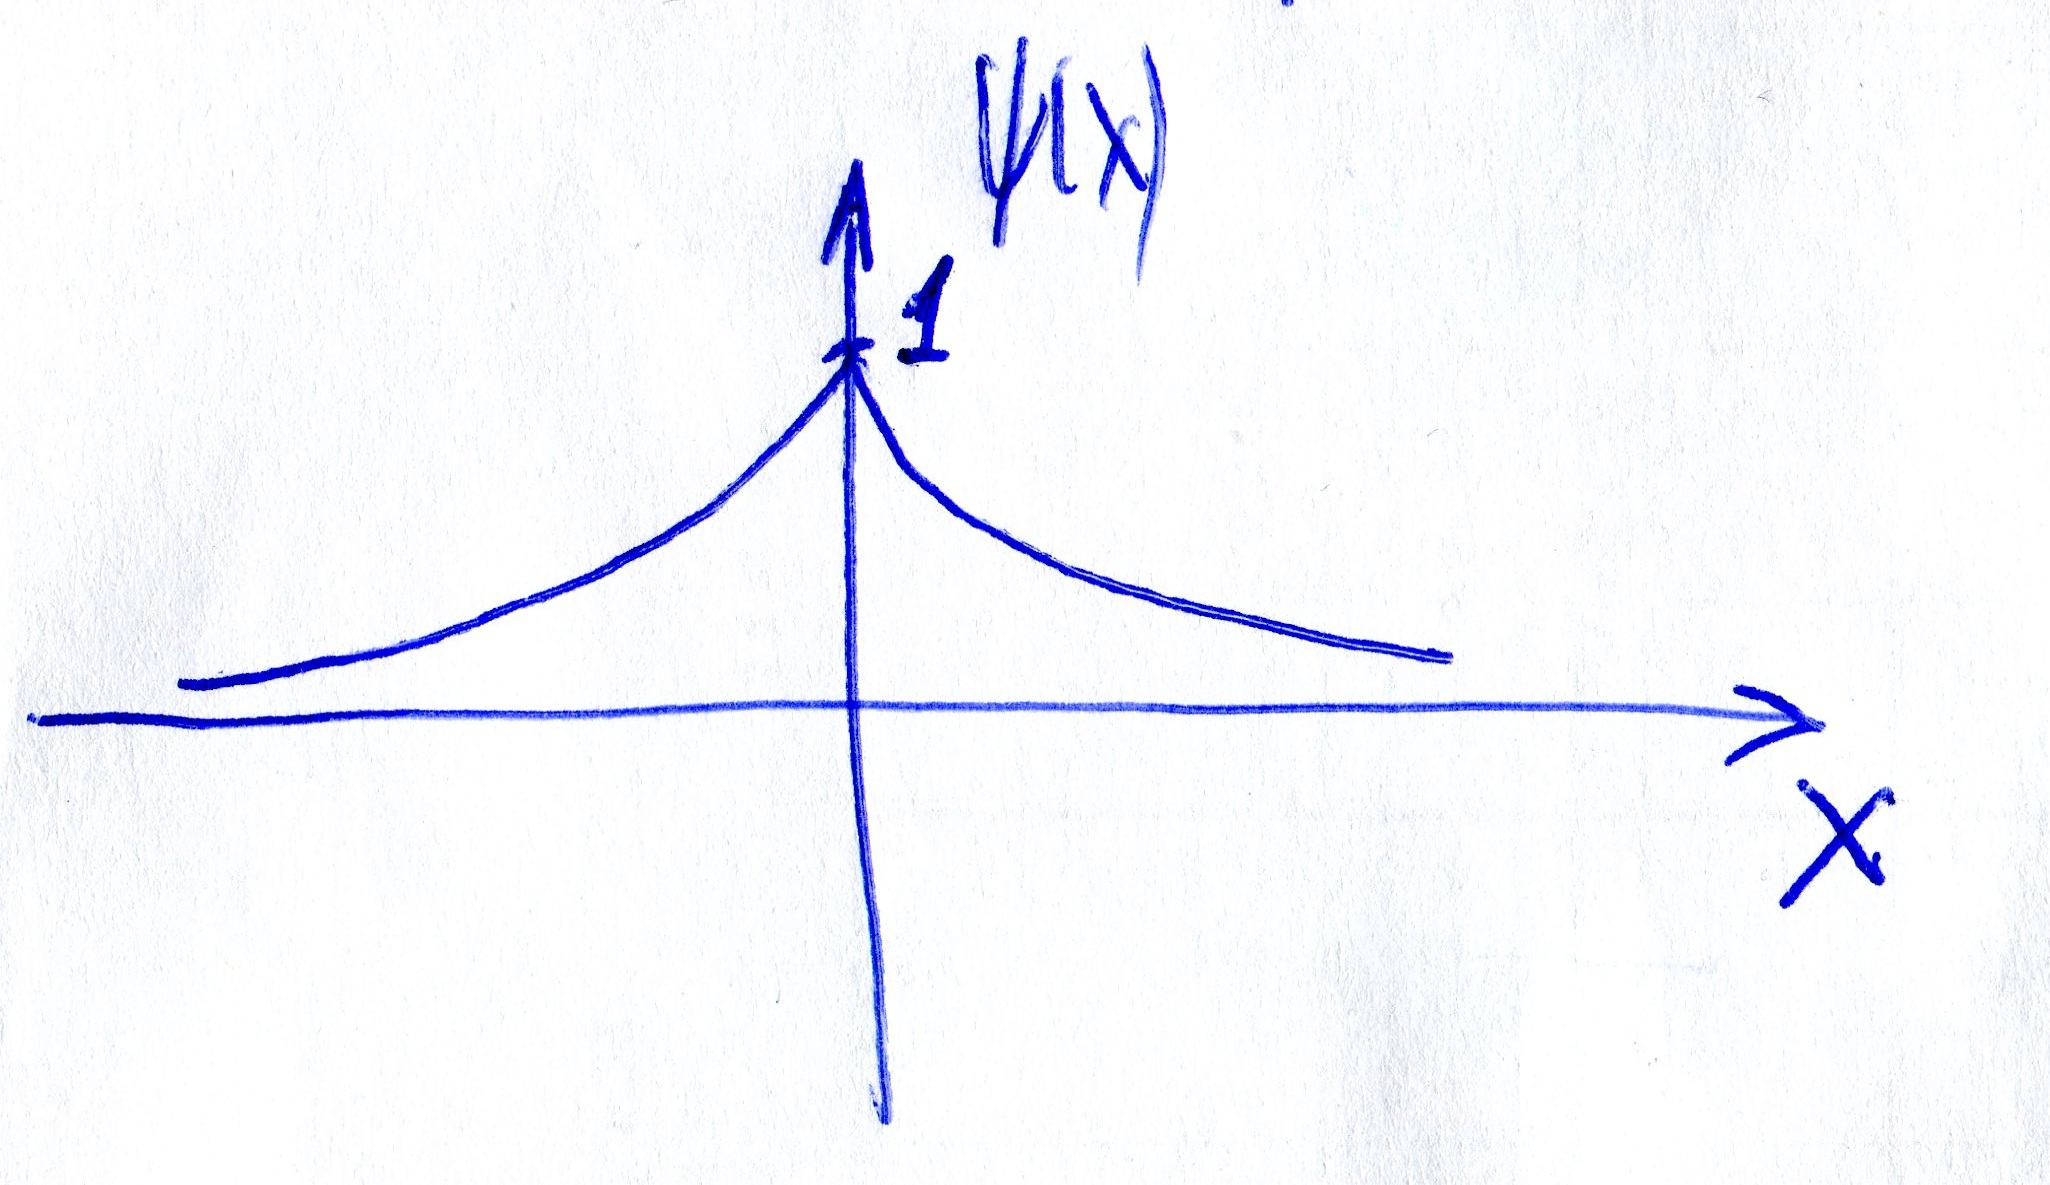
\includegraphics[width=\linewidth]{fig/fig73}
% \caption{}
% \vspace{-17pt}
% \end{wrapfigure}

$\Psi_0(x)=C\Psi(x)$ - нормировочная функция.

$$\int_{-\infty}^{+\infty}|\Psi_0(x)|dx = \int_{-\infty}^{+\infty}|\Psi(x)|^2C^2dx=1$$

$$\int_{-\infty}^{+\infty} e^{-2u|x|}dx=\int_{-\infty}^{0} e^{2ux}dx+\int_{0}^{+\infty} e^{-2ux}dx=\frac{1}{u}$$
$$\frac{C^2}{u}=1 \Longrightarrow C=\sqrt{u}$$
$$\Psi_0(x)=\sqrt{u}\exp{-u|x|}$$
\begin{gather*}
 \Psi(p)=\frac{1}{\sqrt{2\pi \hbar}}\int_{-\infty}^{+\infty} \Psi_0(x) e^{\frac{-ipx}{\hbar}}dx=\frac{\sqrt{u}}{\sqrt{2\pi \hbar}}\int_{-\infty}^{+\infty} e^{-u|x|} e^{\frac{-ipx}{\hbar}}dx=\\
 \sqrt{\frac{u}{2\pi \hbar}}\int_{-\infty}^{+\infty} e^{-(u|x|+\frac{ipx}{\hbar})}dx
\end{gather*}

Когда $x>0$:
$$\int_{0}^{+\infty} e^{-(ux+\frac{-ipx}{\hbar})}dx=\int_{0}^{+\infty} e^{-x(u+\frac{ip}{\hbar})}dx=-\frac{1}{u+\frac{ip}{\hbar}}e^{-x(u+\frac{ip}{\hbar})} \bigg|_0^{+\infty}=\frac{\hbar}{\hbar u+ip}$$

Когда $x<0$:
$$\int_{-\infty}^{0} e^{-(-ux+\frac{-ipx}{\hbar})}dx=\int_{-\infty}^{0} e^{-x(-u+\frac{ip}{\hbar})}dx=-\frac{1}{-u+\frac{ip}{\hbar}}e^{-x(-u+\frac{ip}{\hbar})} \bigg|_{-\infty}^0=-\frac{\hbar}{-\hbar u+ip}$$

$$\frac{\hbar}{\hbar u+ip}-\frac{\hbar}{-\hbar u+ip}=...=\frac{2\hbar ^2u}{p^2+\hbar ^2u^2}$$


$$\Psi(p)=\sqrt{\frac{u}{2\pi \hbar}} \cdot \frac{2\hbar ^2u}{p^2+\hbar ^2u^2}$$

% \begin{wrapfigure}{l}{0.3\linewidth}
% 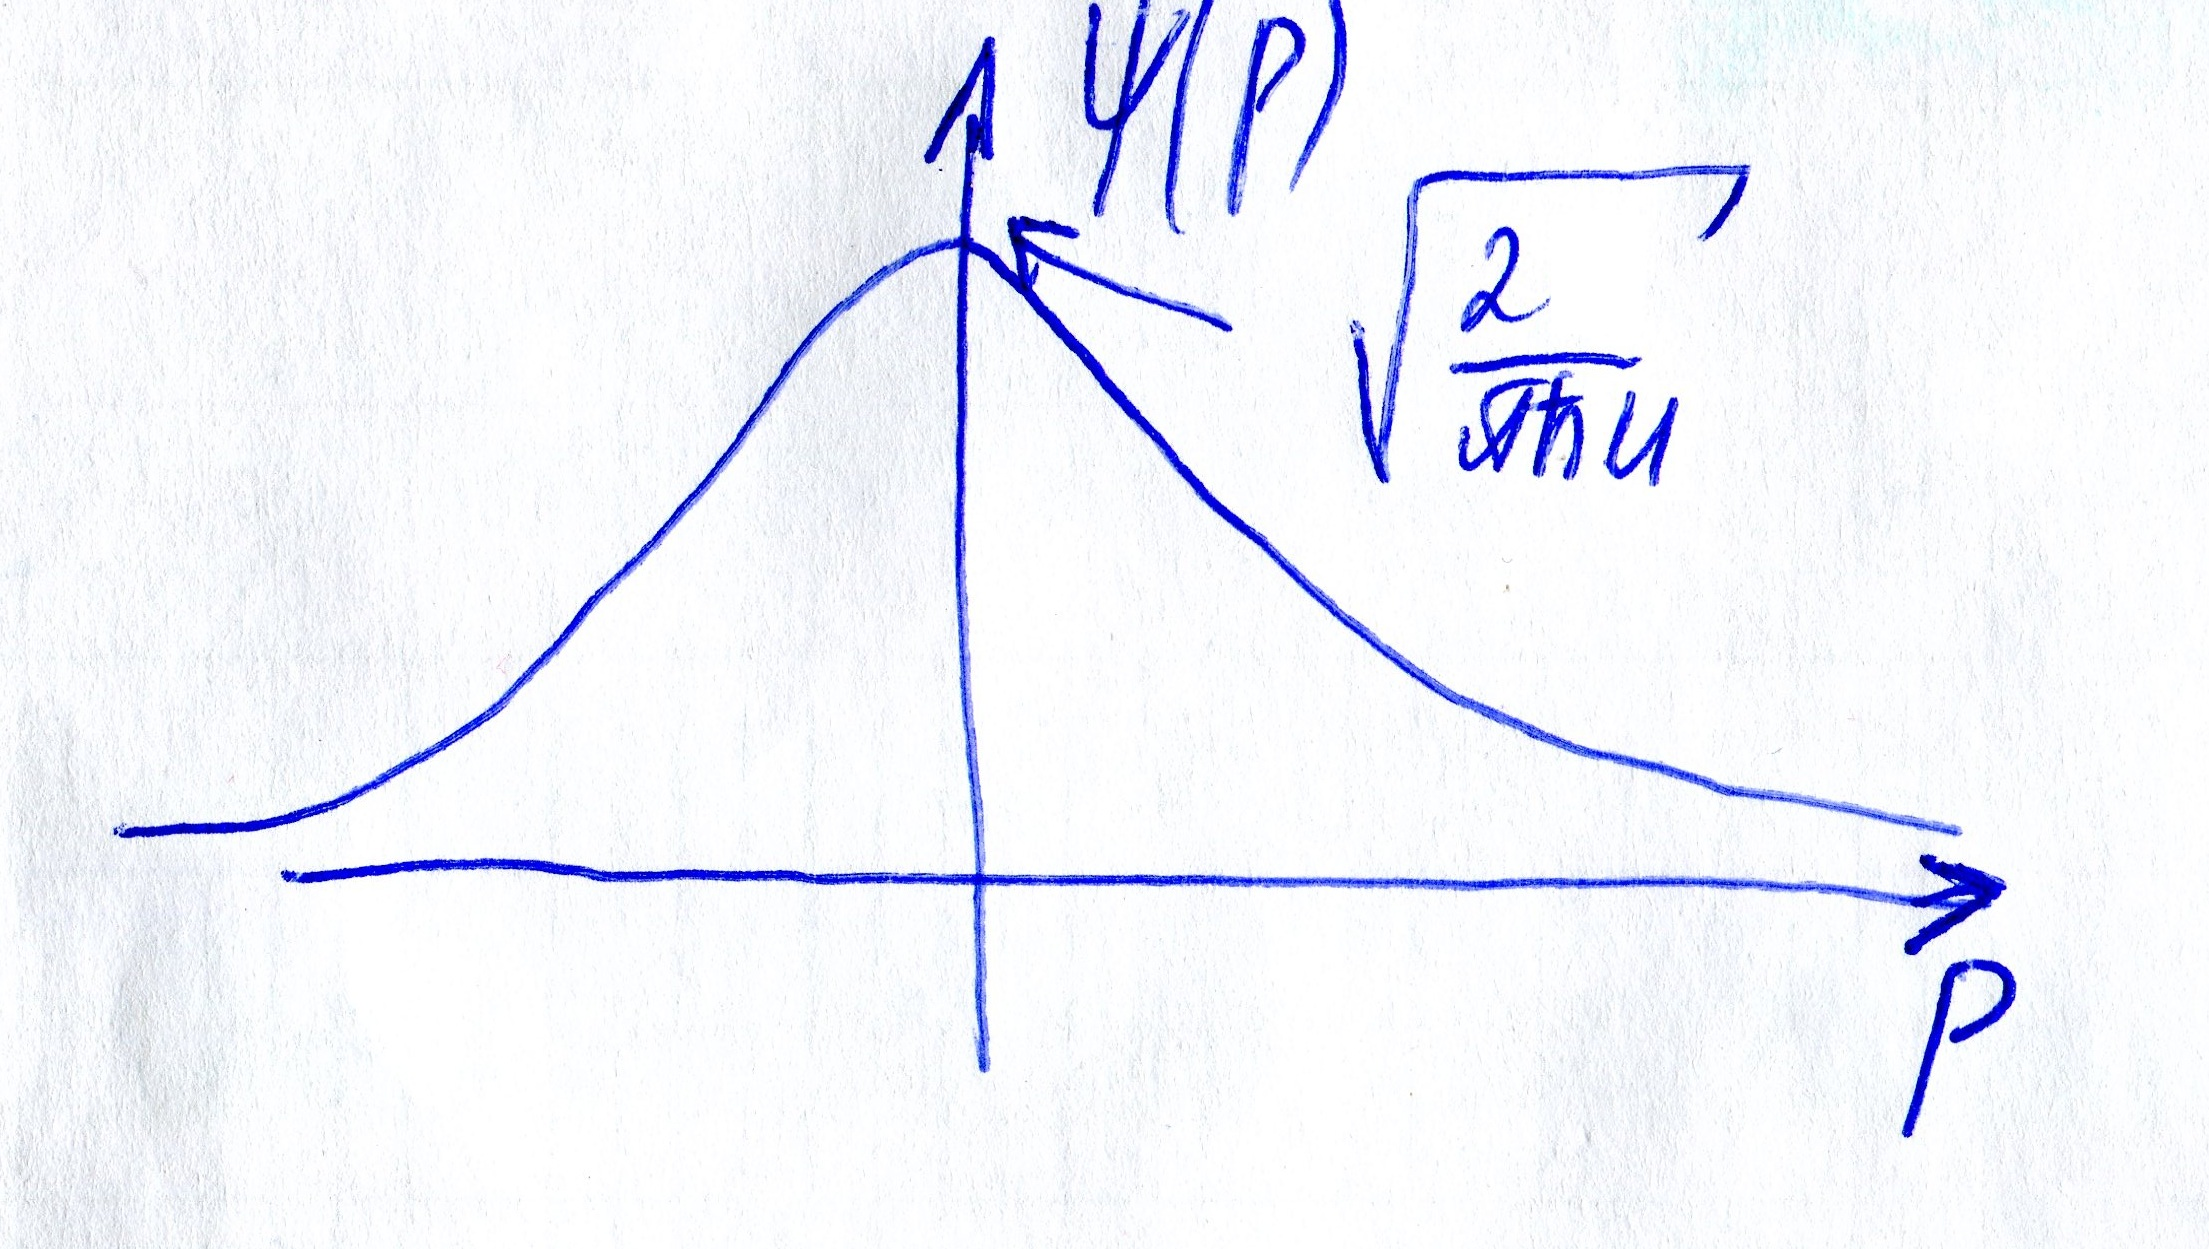
\includegraphics[width=\linewidth]{fig/fig731}
% \caption{}
% \vspace{-17pt}
% \end{wrapfigure}

 Ширина находится на уровне половины от максимума.
 $$\Psi(p=0)=\sqrt{\frac{2}{u\pi \hbar}}$$

 \begin{gather*}
 \Psi(p)=\sqrt{\frac{u}{2\pi \hbar}} \cdot
 \frac{2\hbar ^2u}{(1+\frac{p^2}{\hbar ^2u^2})\hbar ^2u^2}\\
 =\sqrt{\frac{1}{2\pi \hbar u}} \cdot \frac{2}{(1+\frac{p^2}{\hbar ^2u^2})}=\sqrt{\frac{2}{u\pi \hbar}} \cdot \frac{1}{(1+\frac{p^2}{\hbar ^2u^2})}=\Psi(p=0)\cdot \frac{1}{(1+\frac{p^2}{\hbar ^2u^2})} 
 \end{gather*}

 $$\Psi(p^*)=\frac{\Psi(p=0)}{2}$$
 $$\frac{1}{(1+\frac{p^{*2}}{\hbar ^2u^2})}=\frac12 \Longrightarrow p^*=\pm \hbar u $$ 
 $$\Delta p=2\hbar u$$

Найдем $\Delta x$ на уровне $e^{-1}$

$$\Psi(x^*)=\frac{\Psi(p=0)}{e} \Longrightarrow \exp{-u|x^*|}=\exp{-1} \Longrightarrow x^*=\pm \frac{1}{u}$$
 $$\Delta x=\frac{2}{u}$$
 $$\Delta x \cdot \Delta p= 4\hbar$$
<<<<<<< HEAD
 Соотношение неопределенностей позволяет проверить правильность решения. Произведение должно быть равно $\hbar$ с точностью до числового множителя.
=======
 Соотношение неопределенностей позволяет проверить правильность решения. Произведение должно быть равно $\hbar$ с точностью до числового множителя.
>>>>>>> master
